% =====================================================================
%  BÀI BÁO TÓM TẮT ĐỀ TÀI (2 cột, 6 đến 8 trang)
%  Theo "Hướng dẫn cách trình bày bài viết đăng trên Tạp chí Khoa học Giáo dục Kỹ thuật" (HCMUTE):
%  A4, Times 12, lề trên/dưới 1,5 cm, trái 2,5 cm, phải 2 cm, 2 cột cách nhau 0,5 cm,
%  dãn đoạn 6 pt, dòng đơn; đề mục chính IN HOA ĐẬM, đề mục phụ thường đậm;
%  tựa Việt in hoa đậm, cỡ 14; tác giả đậm, đơn vị nghiêng; chỉ có tóm tắt tiếng Việt;
%  tài liệu tham khảo đánh số theo thứ tự trích dẫn.
%  BẢN CẬP NHẬT (_v2): thêm điện thoại phổ thông TCL T506T, 85 thẻ an toàn, vị trí GPS và bản đồ ngoại tuyến.
%  Bản gốc vieedge_paper.tex giữ nguyên. Số đo TCL lấy từ ../so_lieu_tcl.tex (sinh bởi ../make_tcl.py).
%  Biên dịch (2 lần): pdflatex -jobname="24119068_Huỳnh Lê Thành Nhân_Report_v2" vieedge_paper_v2.tex
% =====================================================================
\documentclass[a4paper,12pt,twocolumn]{article}
\usepackage[T5]{fontenc}
\usepackage[utf8]{inputenc}
\usepackage[vietnamese]{babel}
\usepackage{mathptmx}
\usepackage[scaled=.92]{helvet}
\usepackage[a4paper,top=1.5cm,bottom=1.5cm,left=2.5cm,right=2.0cm,footskip=.75cm]{geometry}
\usepackage{graphicx,booktabs,array,xcolor,amsmath,amssymb,microtype,tikz,enumitem,fancyhdr}
\usepackage[font=small,labelfont=bf,labelsep=period,skip=4pt]{caption}
\usepackage[hidelinks,pdftitle={VieEdge-Voice: Trợ lý hỏi đáp bằng giọng nói tiếng Việt chạy hoàn toàn offline trên thiết bị biên},pdfauthor={Huỳnh Lê Thành Nhân (24119068), Nguyễn Đoàn Hoàng Ngân (24119064)},unicode]{hyperref}
\usepackage{stfloats}
\usepackage{balance}
\usepackage{titlesec}
\usetikzlibrary{arrows.meta,positioning,calc}
% Thông tin chung cho bài báo và poster: sửa một chỗ ở đây.
\newcommand{\tenviet}{VieEdge-Voice: Trợ lý hỏi đáp bằng giọng nói tiếng Việt chạy hoàn toàn offline trên thiết bị biên}
\newcommand{\TENVIET}{VIEEDGE-VOICE: TRỢ LÝ HỎI ĐÁP BẰNG GIỌNG NÓI TIẾNG VIỆT CHẠY HOÀN TOÀN OFFLINE TRÊN THIẾT BỊ BIÊN}
\newcommand{\tenanh}{VieEdge-Voice: a fully offline Vietnamese voice question-answering assistant on edge devices}
\newcommand{\svmot}{Huỳnh Lê Thành Nhân}
\newcommand{\mssvmot}{24119068}
\newcommand{\svhai}{Nguyễn Đoàn Hoàng Ngân}
\newcommand{\mssvhai}{24119064}
\newcommand{\emailmot}{24119068@student.hcmute.edu.vn}
\newcommand{\truong}{Trường Đại học Công nghệ Kỹ thuật Thành phố Hồ Chí Minh}
\newcommand{\khoa}{Khoa Đào tạo tiên tiến}
\definecolor{xanhute}{HTML}{0272BC}
\definecolor{doute}{HTML}{D3202A}
\definecolor{dam}{HTML}{0B3C78}

% Sinh tự động bởi make_tcl.py từ results/phone/tcl; không sửa tay.
\newcommand{\tclChip}{Helio P22 (MT6762), 8 lõi Cortex-A53}
\newcommand{\tclRam}{4 GB}
\newcommand{\tclParity}{2.474/2.474}
\newcommand{\tclParityMs}{30\,ms}
\newcommand{\tclSafeOk}{20/24}
\newcommand{\tclSafeOkB}{20/24}
\newcommand{\tclSafeMed}{1,43}
\newcommand{\tclSafeHi}{1,67}
\newcommand{\tclSafeMax}{1,75}
\newcommand{\tclSttMed}{1,33}
\newcommand{\tclFourMed}{1,53}
\newcommand{\tclFourOk}{20/24}
\newcommand{\tclGreedyMed}{1,33}
\newcommand{\tclGrOk}{19/24}
\newcommand{\tclSttNote}{3 luồng 1,43\,s, 4 luồng 1,53\,s, 4 luồng không thiên vị từ khoá 1,33\,s (19/24 đúng thẻ).}
\newcommand{\tclLoadA}{68}
\newcommand{\tclLoadB}{100}
\newcommand{\tclTokA}{3,1}
\newcommand{\tclTokB}{1,8}
\newcommand{\tclAnsA}{12,64}
\newcommand{\tclAnsB}{22,53}
\newcommand{\tclFirstA}{1,99}
\newcommand{\tclFirstB}{2,03}
\newcommand{\tclPssA}{1,3}
\newcommand{\tclPssB}{2,0}
\newcommand{\tclTempA}{35,5}
\newcommand{\tclTempB}{36,5}
\newcommand{\tclNqa}{8}
\newcommand{\tclNqb}{8}
\newcommand{\tclAnsRag}{23,18}
\newcommand{\tclTtftRag}{11,6}
\newcommand{\tclPromptRag}{106}
\newcommand{\tclTtftA}{2,9}
\newcommand{\tclAnsEight}{72,51}
\newcommand{\tclTokEight}{1,2}
\newcommand{\tclBest}{4 luồng, không thiên vị}
\newcommand{\tclTakeaway}{Máy phổ thông vẫn trả lời được offline, nhưng chậm: mô hình 0,8 tỉ cho câu trả lời thật sau 12,64\,s (trung vị, 8 câu, tắt tra cứu), bật tra cứu thì 23,18\,s vì CPU chỉ nạp khoảng 9 token prompt mỗi giây; mô hình 2 tỉ sau 22,53\,s. Câu khẩn cấp không qua LLM nên vẫn có tiếng sau 1,43\,s.}

% Sinh tự động bởi make_hai_may.py; không sửa tay.
\newcommand{\hmAsrF}{65}
\newcommand{\hmAsrT}{889}
\newcommand{\hmAsrRtfF}{0,022}
\newcommand{\hmAsrRtfT}{0,305}
\newcommand{\hmTtsF}{270}
\newcommand{\hmTtsT}{2274}
\newcommand{\hmTtsRtfF}{0,087}
\newcommand{\hmTtsRtfT}{0,722}
\newcommand{\hmSafeMsF}{3,0}
\newcommand{\hmSafeMsT}{27,1}
\newcommand{\hmPpF}{454}
\newcommand{\hmPpT}{10,8}
\newcommand{\hmTgF}{79,5}
\newcommand{\hmTgT}{4,6}
\newcommand{\hmPpBF}{196}
\newcommand{\hmPpBT}{4,3}
\newcommand{\hmTgBF}{28,2}
\newcommand{\hmTgBT}{2,2}
\newcommand{\hmLoadF}{5}
\newcommand{\hmLoadT}{68}
\newcommand{\hmSafeF}{0,48}
\newcommand{\hmSafeT}{1,43}
\newcommand{\hmSafeOkF}{20/24}
\newcommand{\hmSafeOkT}{20/24}
\newcommand{\hmAnsF}{1,4}
\newcommand{\hmFirstF}{0,59}
\newcommand{\hmTtftF}{0,2}
\newcommand{\hmPssF}{1,9}
\newcommand{\hmAnsT}{12,6}
\newcommand{\hmFirstT}{1,99}
\newcommand{\hmTtftT}{2,9}
\newcommand{\hmPssT}{1,3}
\newcommand{\hmSpeedup}{9}

\graphicspath{{../figures/}}
\addto\captionsvietnamese{\renewcommand{\figurename}{Hình}\renewcommand{\tablename}{Bảng}\renewcommand{\refname}{}}
\setlength{\columnsep}{0.5cm}
\setlength{\parindent}{0pt}
\setlength{\parskip}{6pt}
\setlength{\textfloatsep}{8pt plus 2pt minus 2pt}
\setlength{\floatsep}{8pt plus 2pt minus 2pt}
\setlength{\dbltextfloatsep}{8pt plus 2pt minus 2pt}
\setlength{\abovecaptionskip}{4pt}
\pagestyle{fancy}\fancyhf{}\renewcommand{\headrulewidth}{0pt}
\fancyfoot[C]{\small\thepage}
\titleformat{\section}{\normalfont\normalsize\bfseries}{\thesection.}{.4em}{\MakeUppercase}
\titlespacing*{\section}{0pt}{10pt}{2pt}
\titleformat{\subsection}{\normalfont\normalsize\bfseries}{\thesubsection.}{.4em}{}
\titlespacing*{\subsection}{0pt}{6pt}{0pt}
\setlist{itemsep=1pt,topsep=-3pt,parsep=0pt,leftmargin=1.5em}
\newcolumntype{R}[1]{>{\raggedleft\arraybackslash}p{#1}}
\newcolumntype{L}[1]{>{\raggedright\arraybackslash}p{#1}}
\newcommand{\vso}[1]{\ensuremath{#1}}
\hyphenpenalty=1500 \emergencystretch=1.2em
\sloppy

\begin{document}
\twocolumn[{%
\noindent
\includegraphics[height=8.5mm]{logo_hcmute.png}\hfill
\raisebox{3mm}{\small\itshape Báo cáo tóm tắt đề tài dự thi}\par\vspace{5pt}
\begin{center}
{\fontsize{14}{17}\selectfont\bfseries \TENVIET\par}
\end{center}
\vspace{3pt}
\begin{flushright}\setlength{\parskip}{0pt}
\textbf{\svmot}$^{*}$ (MSSV \mssvmot), \textbf{\svhai} (MSSV \mssvhai)\\
\textit{\khoa, \truong}
\end{flushright}
\vspace{1pt}
\noindent\textbf{TÓM TẮT}\par
\noindent Các trợ lý giọng nói phổ biến phụ thuộc vào điện toán đám mây, nên ngừng hoạt động khi mất kết nối và phải truyền giọng nói của người dùng ra khỏi thiết bị. Bài báo khảo sát liệu một thiết bị biên có thể nhận dạng, xử lý và trả lời câu hỏi bằng tiếng Việt mà không cần Internet, với độ trễ đủ thấp cho hội thoại hay không. VieEdge-Voice là đường ống xử lý ngoại tuyến (offline) đầu cuối gồm nhận dạng giọng nói Zipformer, tra cứu Wikipedia cục bộ, mô hình ngôn ngữ lớn (LLM) lượng tử hoá và tổng hợp tiếng nói Piper, được triển khai trên Raspberry Pi 5 chạy Yocto PREEMPT\_RT, trên ứng dụng Android dùng NPU của Galaxy Z Fold7 và trên điện thoại phổ thông TCL T506T chỉ có CPU. Tỉ lệ lỗi từ (WER) trên tập VIVOS là 0,041. Trên Fold7, mô hình 2 tỉ tham số bắt đầu phát nội dung trả lời sau 1,53\,s kể từ khi người dùng nói xong, kể cả khi bật tra cứu; câu hỏi có sẵn được xử lý qua nhánh nhanh trên Pi với độ trễ 0,52\,s. So sánh trên cùng phần cứng cho thấy Yocto-RT giảm đỉnh jitter của lõi xử lý âm thanh 19\% đến 28\% nhưng không làm tăng tốc độ suy luận. Cho kịch bản mất kết nối khi thiên tai, bộ 85 thẻ hướng dẫn sơ cứu, ứng phó thiên tai và an toàn có trích dẫn nguồn được chọn đúng cho 97\% đến 100\% câu hỏi dạng văn bản trên ba tập thử độc lập, nhờ đó mô hình không phải tự sinh lời khuyên y tế; phản hồi âm thanh đầu tiên cho câu hỏi khẩn cấp có sau \hmSafeF\,s trên Fold7 và \hmSafeT\,s trên TCL. Ứng dụng còn định vị GPS và hiển thị bản đồ ngoại tuyến. Các phép đo sử dụng câu hỏi soạn sẵn và giọng đọc tổng hợp; đánh giá với giọng nói thực là bước tiếp theo.

\vspace{2pt}
\noindent\textbf{Từ khóa:} trợ lý giọng nói; tiếng Việt; thiết bị biên; NPU; mô hình ngôn ngữ lớn; PREEMPT\_RT.

\vspace{8pt}
}]
\thispagestyle{fancy}

\section{Giới thiệu}
Trong hội thoại, khoảng lặng giữa hai lượt lời rất ngắn, và chênh lệch giữa các ngôn ngữ chỉ khoảng 250\,ms quanh giá trị trung bình~\cite{stivers}. Do đó, độ trễ phản hồi là một tiêu chí đánh giá quan trọng của trợ lý giọng nói, bên cạnh độ chính xác. Các hệ thống chạy trên đám mây đạt độ trễ thấp nhờ máy chủ có năng lực tính toán lớn, nhưng phụ thuộc vào kết nối mạng và phải truyền giọng nói ra khỏi thiết bị. Kết nối mạng lại thường gián đoạn đúng vào lúc cần thiết nhất: bão lũ, sạt lở làm mất sóng di động và điện lưới, trong khi người dân cần thông tin sơ cứu hoặc thoát hiểm ngay lập tức. Đây là kịch bản sử dụng chính của đề tài.

Triển khai bài toán này trên thiết bị biên cho tiếng Việt gặp ba thách thức. Thứ nhất, các mô hình nhận dạng đa ngôn ngữ có độ chính xác thấp với tiếng Việt: Whisper-tiny~\cite{whisper} có WER 0,53 trên VIVOS trong phép đo của chúng tôi, còn các mô hình tinh chỉnh như PhoWhisper~\cite{phowhisper} vẫn phải đánh đổi giữa kích thước và độ chính xác. Thứ hai, đường ống nối tiếp cộng dồn độ trễ vì mỗi khối phải chờ khối trước~\cite{chipchat}. Thứ ba, mỗi nền tảng có giới hạn riêng: Hailo-8L chỉ hỗ trợ đồ thị tính toán có kích thước cố định, CPU của Pi~5 xử lý prompt chậm, còn NPU điện thoại đòi hỏi chuỗi công cụ của nhà sản xuất.

MELT~\cite{melt} đánh giá LLM trên điện thoại nhưng chỉ xét riêng khối LLM. ChipChat~\cite{chipchat} đạt độ trễ dưới một giây trên Mac Studio bằng kiến trúc xếp tầng, trên phần cứng mạnh hơn nhiều. Theo hiểu biết của chúng tôi, chưa có công bố nào đo độ trễ đầu cuối cho tiếng Việt, từ khi người dùng nói xong đến khi nghe được câu trả lời, trên cả máy nhúng lẫn NPU điện thoại với cùng một quy ước đo.

Đóng góp của đề tài gồm: (i) đường ống ngoại tuyến đo được từng chặng, chạy thực tế trên hai nền tảng (Mục~\ref{sec:system}); (ii) phân tích cơ cấu độ trễ và các biện pháp giảm độ trễ, kèm phép đo bật/tắt từng biện pháp (Mục~\ref{sec:latency}); (iii) so sánh Pi OS và Yocto-RT trên cùng bo mạch có kiểm định thống kê (Mục~\ref{sec:os}); (iv) so sánh CPU, GPU, NPU và báo cáo các kết quả không thành công kèm số đo (Mục~\ref{sec:platform} và \ref{sec:negative}); (v) bộ thẻ sơ cứu và ứng phó thiên tai có trích dẫn nguồn, kèm bộ so khớp câu hỏi được đánh giá trên tập thử độc lập (Mục~\ref{sec:safety}).

\section{Hệ thống và phương pháp}\label{sec:system}
\subsection{Phần cứng}
Nền tảng nhúng là Raspberry Pi 5 8\,GB (4 lõi Cortex-A76, có lệnh dotprod, không có i8mm) gắn Hailo-8L, chạy ảnh Yocto scarthgap với nhân Linux 6.12 PREEMPT\_RT. Nền tảng di động là Samsung Galaxy Z Fold7 (Snapdragon 8 Elite, Hexagon v79, GPU Adreno, Android 16). Để đánh giá trên thiết bị phổ thông, chúng tôi thử nghiệm thêm trên TCL T506T (MediaTek \tclChip, \tclRam{} RAM, Android 13). Bản llama.cpp cho Snapdragon dùng tập lệnh ARMv8.7 nên bị dừng do lệnh không hợp lệ (SIGILL) trên Cortex-A53; vì vậy ứng dụng có thêm một bản dựng ARMv8.0 chỉ dùng CPU. Sản phẩm gồm ứng dụng Android viết bằng Kotlin chạy toàn bộ đường ống trên thiết bị, có thêm chế độ dùng điện thoại làm micro và loa cho Pi qua WebSocket (câu có sẵn được phát sau khoảng 0,59\,s, không xảy ra xrun); ảnh Yocto tái tạo được từ cấu hình; và bảng điều khiển web hiển thị văn bản nhận dạng, câu trả lời và thời gian từng chặng.

\subsection{Đường ống}
Hình~\ref{fig:arch} là lưu đồ xử lý một lượt hỏi. Silero VAD~\cite{silero} phát hiện tiếng nói và xác định điểm kết thúc phát ngôn sau 400\,ms im lặng. Mô hình Zipformer~\cite{zipformer} tiếng Việt 30 triệu tham số~\cite{zipvi}, chạy INT8 trên CPU qua sherpa-onnx~\cite{sherpa}, chuyển lời nói thành văn bản kèm điểm tin cậy; với câu dưới ngưỡng tin cậy, hệ thống đề nghị người dùng nói lại. Câu hỏi sau đó được chuyển tới nhánh nhanh hoặc nhánh tra cứu kết hợp LLM. Khối tách câu chuyển câu đầu tiên sang khối tổng hợp tiếng nói (TTS) ngay khi đủ số từ; văn bản được chuẩn hoá (số, ngày, đơn vị) rồi tổng hợp bằng Piper~\cite{piper}, một bộ tổng hợp dựa trên VITS~\cite{vits}.

\begin{figure*}[t]
\centering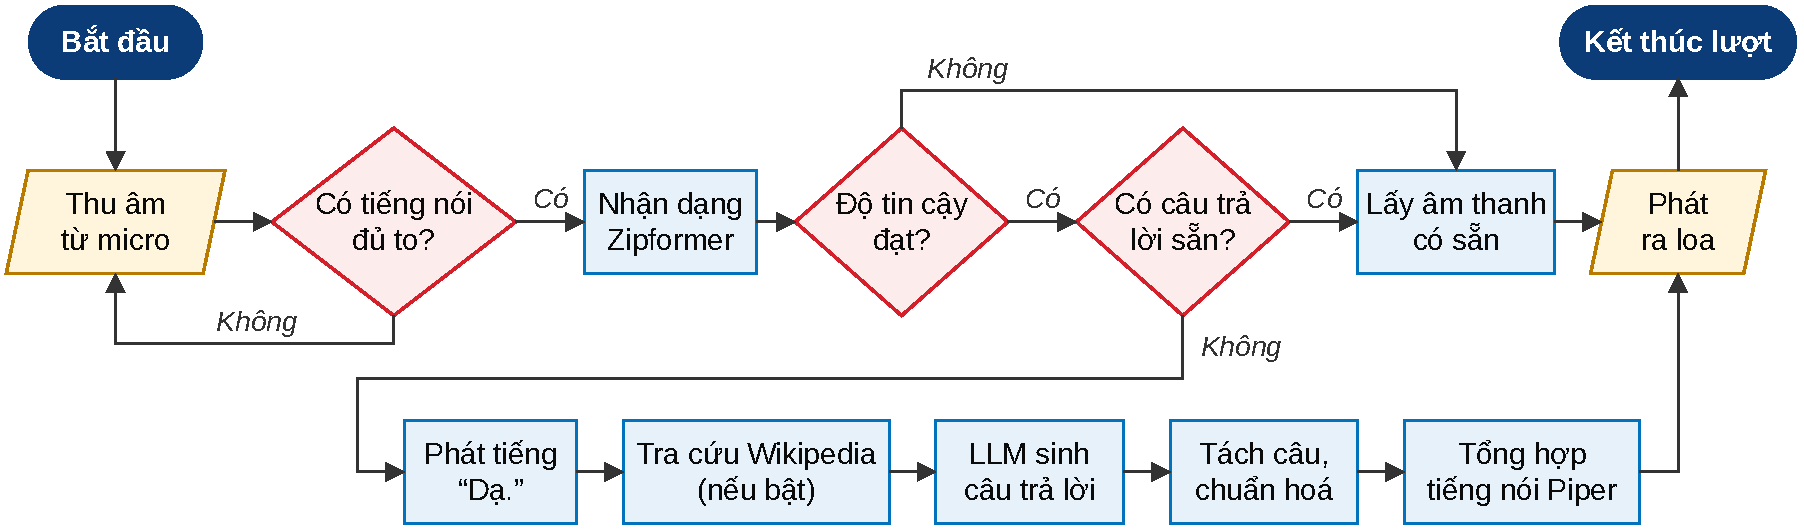
\includegraphics[width=\textwidth]{luu_do.pdf}
\caption{Lưu đồ xử lý một lượt hỏi. Câu không đủ tin cậy và câu có sẵn đều dùng âm thanh tổng hợp sẵn (lần lượt là lời đề nghị nói lại và câu trả lời), không qua LLM. Các câu còn lại qua tra cứu, LLM và TTS theo cơ chế luồng (streaming), nên âm thanh đầu tiên có thể được phát trước khi LLM sinh xong câu trả lời. Cùng lưu đồ chạy trên Pi 5 (âm thanh ở lõi 3, phần còn lại ở lõi 0 đến 2) và trên Fold7 (LLM ở NPU).}\label{fig:arch}
\end{figure*}

Tra cứu dùng 200.000 bài Wikipedia tiếng Việt (1,7 triệu đoạn) lưu trong SQLite FTS5~\cite{fts5}, xếp hạng BM25, chèn đoạn trích 240 ký tự vào câu hỏi theo cách làm của RAG~\cite{rag}. Tệp chỉ mục 1,4\,GB dùng chung cho Pi và điện thoại.

\subsection{LLM và lượng tử hoá}
LLM chạy bằng llama.cpp~\cite{llamacpp} (cùng một phiên bản mã nguồn trên mọi thiết bị). Chúng tôi tinh chỉnh LoRA~\cite{lora} các mô hình Qwen3.5~\cite{qwen} bản 0,8 tỉ và 2 tỉ tham số trên 3.464 cặp hỏi đáp tiếng Việt được sinh và kiểm tra tự động, nhằm tạo câu trả lời ngắn gọn, phù hợp với dạng nói. Trên Cortex-A76, định dạng Q4\_0 được llama.cpp sắp xếp lại thành khối 4$\times$4 tương thích lệnh dotprod, nhờ đó nhanh hơn Q4\_K\_M dù cùng 4 bit (trên Pi 5: xử lý prompt 125 so với 88 token/s, sinh 18,2 so với 16,2 token/s) với độ chính xác tương đương trong phạm vi sai số.

\subsection{Giảm độ trễ}
Với câu hỏi qua LLM, độ trễ tới nội dung trả lời là
\begin{equation}
\begin{split}
T ={}& T_{\text{ngắt}} + T_{\text{STT}} + T_{\text{tra cứu}}\\
&+ T_{\text{TTFT}} + T_{\text{câu đầu}} + T_{\text{TTS}}.
\end{split}
\end{equation}
Từ (1), chúng tôi áp dụng ba biện pháp. Thứ nhất là nhánh nhanh: 149 cặp hỏi đáp có sẵn, được so khớp sau khi loại bỏ dấu câu và phát bằng âm thanh tổng hợp sẵn, nên loại bỏ được bốn số hạng cuối. Thứ hai là cắt câu đầu sớm sau 3 từ thay vì 5 từ, giảm $T_{\text{câu đầu}}$ và $T_{\text{TTS}}$. Thứ ba là xác nhận tức thì: phát âm ``Dạ.'' ngay khi có kết quả nhận dạng. Biện pháp cuối chỉ giảm độ trễ cảm nhận, không làm nội dung trả lời đến sớm hơn, nên hai chỉ số được báo cáo riêng.

\subsection{Triển khai trên Android}
Việc chuyển đường ống sang điện thoại gặp ba vấn đề kỹ thuật. Thư viện OpenCL và FastRPC của nhà sản xuất chỉ truy cập được từ tiến trình của ứng dụng, nên \texttt{llama-server} được nạp ngay trong tiến trình qua JNI thay vì chạy như một tiến trình con. SQLite của Android không có FTS5, nên ứng dụng dùng bản SQLite đóng gói riêng. Tệp mô hình được đặt trong vùng lưu trữ riêng của ứng dụng để bộ nạp truy cập được. Các khối tách câu, chuẩn hoá văn bản và nhánh nhanh được viết lại bằng Kotlin từ bản Python trên Pi để hai nền tảng có cùng hành vi.

\subsection{Chống nhận nhầm tiếng ồn}
Khi không có người nói, Zipformer từng nhận dạng một đoạn nhiễu nền 1,3\,s (RMS 0,003) thành một câu có nghĩa. Chúng tôi tắt bộ tự động điều chỉnh độ lợi (AGC) của micro và chỉ chấp nhận đoạn âm thanh thoả mãn
\begin{equation}
\text{RMS}(x) \ge \max(0{,}008;\ 2{,}5\,\hat{n}),
\end{equation}
trong đó $\hat{n}$ là mức nhiễu nền được ước lượng liên tục. Câu chỉ có một từ bị bỏ qua nếu không khớp với nhánh nhanh.

\subsection{Thời gian thực trên Pi}
PREEMPT\_RT~\cite{preemptrt} được dựng bằng Yocto~\cite{yocto}. Tiến trình xử lý âm thanh chạy trên lõi 3 đã được cô lập (\texttt{isolcpus=3 nohz\_full=3 rcu\_nocbs=3}), SCHED\_FIFO mức 80, khoá bộ nhớ. STT, LLM và TTS ở lõi 0 đến 2.

\subsection{Thẻ an toàn đã kiểm duyệt}
Mô hình nhỏ có tỉ lệ ảo giác (thông tin sai) từ 12\% đến 52\% (Mục~\ref{sec:quality}); mức này có thể chấp nhận với câu hỏi kiến thức chung nhưng không chấp nhận được với tình huống khẩn cấp như ``con tôi bị rắn cắn''. Vì vậy câu hỏi khẩn cấp được trả lời bằng thẻ soạn sẵn, không do LLM sinh. Bộ 85 thẻ (sơ cứu, thiên tai và an toàn, tối đa 110 từ mỗi thẻ) được nhóm biên soạn lại từ 82 nguồn trong nước (Cục Quản lý đê điều và Phòng, chống thiên tai, Bộ Y tế, Trung tâm Chống độc Bệnh viện Bạch Mai, Tổng đài 111, Quyết định 2024/QĐ-TTg về số 112) và quốc tế (WHO, CDC, Ready.gov, MedlinePlus, Hội Chữ thập đỏ Úc và các cơ quan khác). Ngoài tình huống tại Việt Nam, bộ thẻ bao gồm cả tình huống ở nước ngoài: sự cố phóng xạ, xả súng, gặp gấu, bão tuyết, bão cát và số điện thoại khẩn cấp của các nước. Mọi nội dung không truy được về nguồn đều bị loại khỏi thẻ. Bản dịch Ready.gov ghi nhầm ngưỡng bỏ thực phẩm là 40\,°C thay vì 40\,°F nên con số này không được dùng.

Bộ so khớp giữ nguyên dấu tiếng Việt, vì khi bỏ dấu thì ``bất tỉnh'' trùng với ``bật tính'' và ``đuối nước'' trùng với ``dưới nước''. Một thẻ được chọn khi câu hỏi chứa một cụm từ khoá của thẻ hoặc một tổ hợp từ (``rắn'' và ``cắn'' ở vị trí bất kỳ trong câu); thẻ cụ thể hơn được ưu tiên. Câu hỏi kiến thức như ``lũ quét hình thành thế nào'' được chuyển cho LLM. Câu hỏi khẩn cấp chưa có thẻ nhận một câu trả lời cố định: chưa có hướng dẫn đã kiểm duyệt, hãy gọi 115 hoặc 112. Khi luật không tìm được thẻ, một bộ phân loại hồi quy logistic (đặc trưng từ đơn và cặp từ, có dấu và không dấu) huấn luyện trên 10.832 câu, gồm cả câu đã qua nhận dạng giọng nói, được dùng bổ sung với ngưỡng xác suất 0,90; ngưỡng được chọn trên tập kiểm định sao cho không phát sinh thêm trường hợp kích hoạt nhầm. Bộ giải mã của Zipformer được tăng trọng số (hotword biasing) cho 1.276 cụm từ khẩn cấp, vì giấy phép của mô hình không cho phép tinh chỉnh. Luật và bộ phân loại được lưu trong tệp dữ liệu, nên bản Python và bản Kotlin cho kết quả giống hệt nhau trên 2.474 câu thử. Câu đầu của mỗi thẻ được tổng hợp sẵn và lưu trên thiết bị để phát ngay.

\subsection{Tính năng và ưu điểm của thiết kế}
Bảng~\ref{tab:feat} liệt kê các tính năng đã hoàn thành trên ba thiết bị. Thiết kế có ba ưu điểm chính: toàn bộ xử lý diễn ra trên thiết bị nên dữ liệu giọng nói không rời máy và hệ thống vẫn hoạt động khi mất Internet; mỗi khối (STT, LLM, TTS, tra cứu, bộ xử lý) được chọn qua cấu hình nên cùng một đường ống chạy được trên Pi và điện thoại; mọi lượt đều ghi mốc thời gian từng chặng nên mỗi tối ưu đều có số đo trước và sau. Ứng dụng còn tích hợp định vị GPS (không cần mạng di động, hiển thị số vệ tinh và sai số, lưu vị trí gần nhất khi mất tín hiệu); tọa độ được hiển thị trên mọi câu trả lời khẩn cấp để cung cấp cho tổng đài 115. Bản đồ ngoại tuyến được tải trước từ OpenFreeMap trong giới hạn 3.000 mảnh mỗi lần theo điều khoản sử dụng của dịch vụ; máy chủ tile.openstreetmap.org cấm tải trước nên không được sử dụng. Trên TCL, vùng 25$\times$25\,km gồm 224 mảnh (30,8\,MB) được tải trong khoảng 45\,s qua Wi-Fi; sau khi tắt Wi-Fi, bản đồ vẫn hiển thị đầy đủ, kể cả các khu vực chưa từng được xem trước đó.

\begin{table}[t]\centering\small
\caption{Các tính năng đã hoàn thành. $\checkmark$: có; $\times$: không có.}\label{tab:feat}
\setlength{\tabcolsep}{3pt}
\begin{tabular}{@{}L{51mm}ccc@{}}\toprule
Tính năng & Pi 5 & Fold7 & TCL\\\midrule
Hỏi đáp tiếng Việt ngoại tuyến & $\checkmark$ & $\checkmark$ & $\checkmark$\\
Nhánh nhanh cho câu hỏi có sẵn & $\checkmark$ & $\checkmark$ & $\checkmark$\\
Tra cứu Wikipedia ngoại tuyến & $\checkmark$ & $\checkmark$ & $\checkmark$\\
Xác nhận tức thì ``Dạ.'' & $\checkmark$ & $\checkmark$ & $\checkmark$\\
Chạm để nói, tự dừng khi im lặng, lọc nhiễu & $\checkmark$ & $\checkmark$ & $\checkmark$\\
Đề nghị nói lại theo độ tin cậy & $\checkmark$ & $\times$ & $\times$\\
Chọn CPU, GPU hoặc NPU cho LLM & $\times$ & $\checkmark$ & $\times$\\
Bảng điều khiển đo từng chặng & $\checkmark$ & $\times$ & $\times$\\
Điện thoại làm micro, loa cho Pi & $\checkmark$ & $\checkmark$ & $\checkmark$\\
Lõi âm thanh thời gian thực & $\checkmark$ & $\times$ & $\times$\\
Thẻ sơ cứu, thiên tai có nguồn & $\checkmark$ & $\checkmark$ & $\checkmark$\\
Vị trí GPS, bản đồ ngoại tuyến & $\times$ & $\checkmark$ & $\checkmark$\\
Lịch sử trò chuyện & $\times$ & $\checkmark$ & $\checkmark$\\\bottomrule
\end{tabular}
\end{table}



\subsection{Giao thức đo}
Mọi độ trễ được tính từ khi người dùng nói xong và bao gồm thời gian chờ xác định điểm kết thúc phát ngôn. Tập câu hỏi gồm 12 đến 16 câu được tổng hợp bằng một giọng khác với giọng của trợ lý và được đưa vào bằng cùng một công cụ cho mọi cấu hình; trên điện thoại, âm thanh được đưa trực tiếp vào ứng dụng, trên Pi được nạp từ tệp. ``Phản hồi đầu'' là thời điểm phát âm thanh đầu tiên, ``nội dung trả lời'' là thời điểm bắt đầu phát phần trả lời chính. Chúng tôi báo cáo trung vị (p50), phân vị 95 (p95), khoảng tin cậy 95\% của trung vị bằng bootstrap (10.000 lần lấy mẫu), và kiểm định Wilcoxon cặp đôi khi so sánh trên cùng bộ câu. WER được đo trên VIVOS~\cite{vivos} với cùng một chương trình. Độ chính xác của LLM được đo bằng Global-MMLU tiếng Việt~\cite{gmmlu} ($n=400$, sai số $\pm 2{,}5$ điểm) và bằng một mô hình lớn hơn đóng vai trò giám khảo trên 345 câu.

\section{Kết quả và thảo luận}
\subsection{Chỉ tiêu và kết quả}
Bảng~\ref{tab:target} đối chiếu kết quả với chỉ tiêu đặt ra trong đề xuất ban đầu. Ba chỉ tiêu đạt, một chỉ tiêu chưa đạt, và phần triển khai trên điện thoại vượt kế hoạch. Nội dung trả lời chưa có chỉ tiêu riêng; p95 của chỉ số này vẫn trên 1,5\,s ở cả hai nền tảng.

\begin{table}[t]\centering\small
\caption{Chỉ tiêu trong đề xuất và kết quả đo.}\label{tab:target}
\setlength{\tabcolsep}{3pt}
\begin{tabular}{@{}L{27mm}L{36mm}l@{}}\toprule
Chỉ tiêu & Kết quả & Đánh giá\\\midrule
Phản hồi đầu p95 dưới 1,5\,s & Pi 1,15\,s; Fold7 1,24\,s & Đạt\\
Không xrun & 0 (chưa thử loa, micro USB) & Đạt\\
STT trên NPU Hailo-8L & cosine 0,84, dưới ngưỡng 0,9 & Chưa đạt\\
Hoàn toàn ngoại tuyến & không cần mạng & Đạt\\
Chạy trên điện thoại & 1,53\,s, có tra cứu & Vượt\\\bottomrule
\end{tabular}
\end{table}

\subsection{Nhận dạng giọng nói}
Trên cùng tập câu VIVOS, WER của Whisper-tiny, PhoWhisper-tiny và Zipformer lần lượt là 0,529, 0,158 và 0,046 với âm thanh sạch; ở nhiễu 5\,dB, PhoWhisper đạt 0,224 và Zipformer 0,059; với câu giọng tổng hợp ($n=120$) là 0,312 và 0,189. WER của Zipformer thấp hơn PhoWhisper-tiny khoảng ba lần với âm thanh sạch và bốn lần ở nhiễu 5\,dB. Trên 300 câu VIVOS, WER của Zipformer là 0,041, thời gian xử lý 29\,ms mỗi câu trên máy tính xách tay (hệ số thời gian thực 0,008). Trên điện thoại, 12 câu tổng hợp cho WER 0,257, so với 0,250 trên máy tính xách tay với cùng các tệp, cho thấy bản Android không làm giảm độ chính xác trong phạm vi mẫu nhỏ này.





Điểm tin cậy của Zipformer phân biệt được câu nhận dạng sai với AUROC 0,84; ngưỡng $-0{,}20$ từ chối 4,7\% số câu. Trên giọng tổng hợp, cơ chế này chặn 4 trong 16 câu ở Yocto và 5 trong 16 câu ở Pi OS, các lượt đó được đề nghị nói lại; chúng tôi chưa xác định được bao nhiêu trong số này thực sự bị nhận dạng sai.

\subsection{Chất lượng câu trả lời}\label{sec:quality}
Điểm do mô hình giám khảo chấm (thang 5) là 3,63 với mô hình 0,8 tỉ và 4,17 với mô hình 2 tỉ; tỉ lệ ảo giác của mô hình 2 tỉ là 0,12. Khi câu hỏi đi qua nhận dạng giọng nói, tỉ lệ ảo giác của mô hình 0,8 tỉ tăng lên 0,52; bật tra cứu giảm tỉ lệ này về 0,30. Lỗi nhận dạng là nguyên nhân chính làm giảm chất lượng: điểm giảm từ 3,64 với câu văn bản xuống 2,73 với câu qua Zipformer, trong đó câu hỏi giọng tổng hợp có WER 0,19.

\subsection{Cơ cấu độ trễ}\label{sec:latency}
Hình~\ref{fig:stages} phân tách trung vị từng chặng của các lượt thực sự đi qua LLM, cùng mô hình 0,8 tỉ trên bốn cấu hình. Trên Pi, phần lớn thời gian nằm ở việc LLM sinh đủ câu đầu và TTS tổng hợp câu đó, không phải ở token đầu tiên. Trên Fold7, NPU và CPU cho cùng 1,4\,s và chặng lớn nhất là chờ kết thúc phát ngôn cộng STT (0,56\,s); token đầu chỉ mất 0,12 đến 0,17\,s, nên tăng tốc LLM thêm khó cải thiện đáng kể tổng độ trễ. Trên TCL, mọi chặng đều dài hơn nhiều lần (tổng 12,2\,s), lớn nhất là LLM sinh câu đầu (4,2\,s) và TTS (3,2\,s).

\begin{figure}[t]
\centering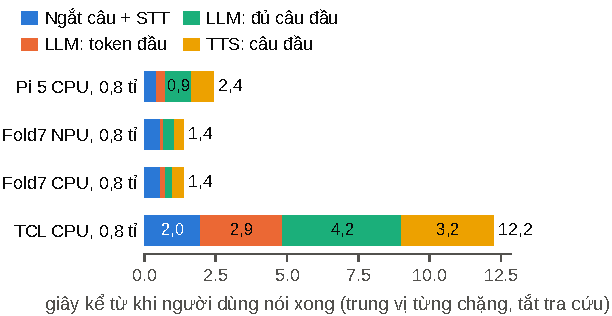
\includegraphics[width=\columnwidth]{stages_v2.pdf}
\caption{Thời gian tới nội dung trả lời theo từng chặng, mô hình 0,8 tỉ, tắt tra cứu. Fold7 và TCL: cùng 8 câu nói, câu đầu tối đa 7 từ; Pi: 12 câu, câu đầu 5 từ (đo tháng 10). Số bên phải là tổng.}\label{fig:stages}
\end{figure}

\begin{figure}[t]
\centering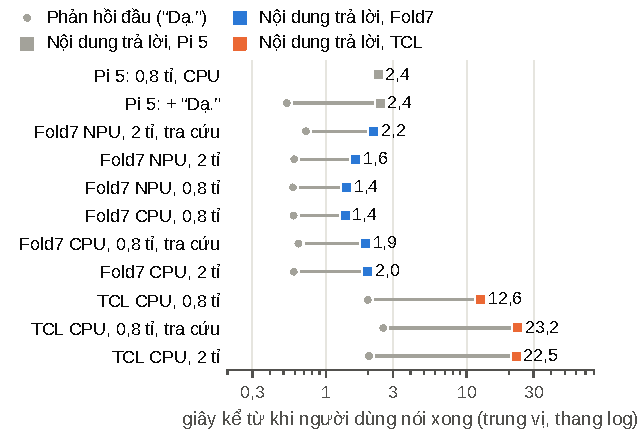
\includegraphics[width=.92\columnwidth]{hai_may_latency.pdf}
\caption{Phản hồi đầu (``Dạ.'') và nội dung trả lời trên ba thiết bị; cùng 8 câu nói cho mọi cấu hình điện thoại, bật ``Dạ.'', không gửi kèm lượt trước; Pi: 12 câu (tháng 10). Thang logarit: TCL chậm hơn Fold7 khoảng \hmSpeedup{} lần với cùng mô hình và cùng CPU. Số bên phải là trung vị thời gian tới nội dung trả lời.}\label{fig:latency}
\end{figure}

Hình~\ref{fig:latency} đặt mọi cấu hình trên cùng một trục: ``Dạ.'' được phát sau khoảng 0,6\,s trên Fold7 và 2,0\,s trên TCL, còn nội dung trả lời có sau 1,4\,s (Fold7) đến 12,6\,s (TCL, 0,8 tỉ) và trên 20\,s khi TCL dùng mô hình 2 tỉ hoặc bật tra cứu. Bảng~\ref{tab:abl} cho kết quả bật/tắt từng biện pháp trên Fold7. Cắt câu đầu từ 5 xuống 3 từ giảm p50 từ 2,03\,s xuống 1,60\,s và p95 từ 3,51\,s xuống 2,38\,s; khoảng tin cậy của p50 còn chồng lấn nên đây mới là xu hướng, chưa phải kết luận chắc chắn. Tăng số luồng TTS và rút ngưỡng im lặng còn 300\,ms không tạo khác biệt vượt khoảng tin cậy, nên cấu hình mặc định giữ 400\,ms để tránh cắt ngang người nói chậm. Nhánh nhanh trên Pi trả lời câu có sẵn sau 0,52\,s, xấp xỉ thời gian chờ kết thúc phát ngôn, và không kích hoạt nhầm với câu nào trong 345 câu hỏi kiến thức của tập thử.

\begin{table}[t]\centering\small
\caption{Bật/tắt từng biện pháp trên Fold7 (2 tỉ, NPU, bật tra cứu và ``Dạ.'', $n=12$ đến 13). Cấu hình: số từ câu đầu, số luồng TTS, ngưỡng im lặng (ms). P.h. đầu: phản hồi đầu (s); nội dung: thời điểm phát nội dung trả lời (s); KTC: khoảng tin cậy 95\% của p50 nội dung. Cấu hình mặc định in đậm.}\label{tab:abl}
\setlength{\tabcolsep}{3pt}
\begin{tabular}{@{}lrrr@{}}\toprule
Cấu hình & P.h. đầu & Nội dung & KTC\\\midrule
5 từ, 3 luồng, 400 & 0,66 & 2,03 & [1,47; 2,19]\\
3 từ, 3 luồng, 400 & 0,66 & 1,60 & [1,39; 1,70]\\
\textbf{3 từ, 4 luồng, 400} & \textbf{0,65} & \textbf{1,53} & [1,47; 1,78]\\
3 từ, 4 luồng, 300 & 0,57 & 1,55 & [1,40; 1,92]\\\bottomrule
\end{tabular}
\end{table}

\subsection{So sánh nền tảng}\label{sec:platform}
Hình~\ref{fig:platform} cho thấy NPU Hexagon xử lý prompt nhanh gấp 16 lần CPU Pi 5 trên cùng tệp mô hình, trong khi CPU điện thoại sinh token nhanh nhất. Nhờ đó, tra cứu gần như không làm tăng độ trễ trên điện thoại: thời gian tra cứu là 96\,ms (p50) và prompt tăng từ 25 lên 107 token, nhưng nội dung trả lời chỉ chậm thêm 0,06\,s (1,69\,s so với 1,75\,s), trong khi cùng tính năng trên Pi làm chậm thêm 1,4 đến 2,8\,s. Với cùng 4 luồng, CPU của TCL xử lý prompt \hmPpT{} token/s và sinh \hmTgT{} token/s, so với \hmPpF{} và \hmTgF{} của Fold7; Cortex-A53 không có lệnh dotprod nên chênh lệch ở xử lý prompt lớn hơn ở sinh token.

\begin{figure}[t]
\centering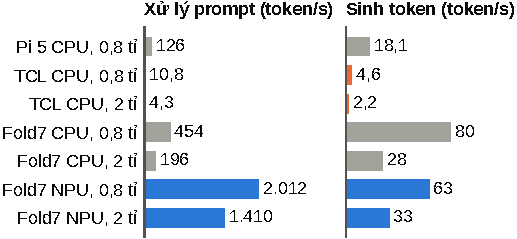
\includegraphics[width=\columnwidth]{platform_v2.pdf}
\caption{\texttt{llama-bench} (prompt 128, sinh 64 token), bản Q4\_0. CPU của hai điện thoại: cùng 4 luồng; TCL dùng bản ARMv8.0. NPU vượt trội ở xử lý prompt; trên TCL, xử lý prompt chậm hơn Fold7 khoảng 42 lần.}\label{fig:platform}
\end{figure}

Trên Fold7, mô hình 0,8 tỉ trả lời nhanh hơn mô hình 2 tỉ khoảng 0,2 đến 0,3\,s (Hình~\ref{fig:latency}) nhưng điểm giám khảo thấp hơn 0,54 điểm (3,63 so với 4,17). Đối với trợ lý hỏi đáp, chúng tôi chọn mô hình 2 tỉ trên NPU làm mặc định vì chất lượng cao hơn và thời gian nạp mô hình ngắn (6 đến 10\,s); GPU Adreno sinh token nhanh hơn (36 so với 26 token/s) nhưng nạp mô hình mất 14 đến 24\,s. Do số lượt ít, thứ tự giữa các cấu hình có kết quả gần nhau chỉ nên được xem là xu hướng.



\subsection{Pi OS và Yocto-RT}\label{sec:os}
Bảng~\ref{tab:os} sử dụng cùng bo mạch, cùng chương trình đo và cùng mô hình Q4\_0. Yocto-RT giảm đỉnh jitter khi tải nặng từ 105 xuống 85\,µs trong 5 phút và từ 127 xuống 92\,µs trong 30 phút (1,8 triệu mẫu), trong khi các phân vị p99 đến p99,99 gần như bằng nhau. Yocto sử dụng ít RAM hơn sau khởi động. Về độ trễ trả lời khi không tải, trung vị của Pi OS thấp hơn 0,42\,s, nhưng so cặp trên cùng 16 câu thì chênh lệch trung vị chỉ là 0,06\,s (khoảng tin cậy $-0{,}08$ đến $0{,}59$\,s, Wilcoxon $p=0{,}40$). Các số liệu này bao gồm cả lượt được đề nghị nói lại; nếu chỉ xét lượt qua LLM thì trung vị là 1,85\,s và 2,44\,s, so cặp 11 câu cho $p=0{,}83$. Với cỡ mẫu này, chúng tôi không thể khẳng định hệ điều hành nào nhanh hơn. Như vậy, lợi ích của Yocto-RT là khả năng cô lập và ảnh hệ thống gọn nhẹ, không phải tốc độ suy luận.

\begin{table}[t]\centering\small
\caption{Pi OS nguyên bản (O0) và Yocto-RT (O4) trên cùng Pi 5, LLM 0,8 tỉ Q4\_0. Yocto 30 phút đo bản Q4\_K\_M.}\label{tab:os}
\setlength{\tabcolsep}{3pt}\footnotesize
\begin{tabular}{@{}lrr@{}}\toprule
Chỉ số & Pi OS & Yocto-RT\\\midrule
Đỉnh jitter, không tải, 5 ph (µs) & 33 & \textbf{13}\\
Đỉnh jitter, tải nặng, 5 ph (µs) & 105 & \textbf{85}\\
Đỉnh jitter, tải nặng, 30 ph (µs) & 127 & \textbf{92}\\
Trả lời, không tải, p50 (s) & 1,60 & 2,02\\
Trả lời, không tải, p95 (s) & 3,62 & 3,78\\
Trả lời, tải nền 4 lõi, p50 (s) & 9,27 & \textbf{6,51}\\
RAM sau khởi động (MB) & 442-538$^{\dagger}$ & \textbf{285}\\
Công suất PMIC, không tải (W) & 3,03 & \textbf{2,78}\\
Xrun mỗi giờ & 0 & 0\\\bottomrule
\end{tabular}\\[1pt]
{\footnotesize $^{\dagger}$ đo ở cấu hình O1.}
\end{table}



\subsection{Nhiệt và công suất}
Trên Fold7, trong 7,5 phút chạy liên tục (62 lượt), nhiệt độ NPU cao nhất là 65\,°C và tốc độ sinh duy trì 25,3 token/s, không có dấu hiệu giảm xung nhịp do nhiệt. Khi chạy bằng pin, toàn máy tiêu thụ 2,2 đến 3,3\,W kể cả màn hình (16 đến 24\,J mỗi lượt); số liệu 2,78\,W của Pi 5 là ước lượng PMIC của bo mạch nên không cùng phạm vi đo.



\subsection{Kịch bản khẩn cấp khi mất kết nối}\label{sec:safety}
Bảng~\ref{tab:safety} trình bày kết quả của bộ so khớp. Tập phát triển được dùng để hiệu chỉnh luật nên không được xem là số đo độc lập. Mỗi lần bổ sung thẻ, nhóm soạn một tập câu thử mới và ghi mã băm của tệp trước khi viết từ khoá cho thẻ, sau đó chạy đánh giá đúng một lần: v2 cho 42 thẻ đầu, v3 cho 60 thẻ, v4 cho 16 thẻ đợt hai và v5 cho 9 thẻ tình huống quốc tế. Với đầu vào văn bản, 97\% đến 100\% câu được chọn đúng thẻ. Khi câu được đọc bằng giọng tổng hợp rồi qua Zipformer, tỉ lệ đúng giảm theo chất lượng giọng: giọng rõ (WER 0,15 đến 0,22) đạt 73\% đến 89\%, giọng kém (WER 0,40 đến 0,44) chỉ còn 42\% đến 48\%. Tăng trọng số từ khoá và bộ phân loại cùng sửa đúng thêm 5 câu mà không làm sai câu nào trên v3 giọng rõ (McNemar $p=0{,}06$) và 7 câu trên v3 giọng kém ($p=0{,}016$); đổi lại có 2 trên 234 câu hỏi thông thường bị nhận nhầm thành câu khẩn cấp. Lần chạy đầu của v4 cho thấy một lỗ hổng: 7 trên 10 câu khẩn cấp chưa có thẻ (đẻ rơi, rết cắn, ngộ độc cá nóc) bị chuyển sang LLM thay vì nhận câu trả lời ``gọi 115''; sau khi mở rộng danh sách từ khẩn cấp, v5 xử lý chấp nhận được 14 trên 20 câu thuộc loại này.

Trên điện thoại, bản Kotlin cho kết quả giống hệt bản Python trên 2.474 câu ở cả Fold7 (2,1\,ms mỗi câu) và TCL (\tclParityMs). Với 24 câu nói chọn ngẫu nhiên, hai máy chọn đúng thẻ như nhau (20/24) và nhận dạng sai cùng các câu, ví dụ ``pin'' thành ``tinh''. Trên Fold7 (bản dựng cuối), khi câu hỏi được đưa vào 1\,s sau khi khởi động trợ lý, phản hồi đầu có sau \hmSafeF\,s (trung vị), chậm nhất 0,61\,s; ở lần khởi động đầu tiên sau khi cài đặt, máy cần khoảng 90\,s để tổng hợp sẵn câu đầu của 85 thẻ, trước thời điểm đó câu khẩn cấp có thể chậm tới 1,7\,s.

\begin{table}[t]\centering\small
\caption{Bộ so khớp thẻ an toàn trên các tập độc lập (khoá trước khi viết luật). Có thẻ: số câu chọn đúng thẻ. Không thẻ: số câu nhận câu trả lời ``gọi 115'' hoặc một thẻ chấp nhận được. Thường: số câu hỏi thông thường bị kích hoạt nhầm. Giọng rõ, kém: câu qua TTS và Zipformer.}\label{tab:safety}
\setlength{\tabcolsep}{1.2pt}\footnotesize
\begin{tabular}{@{}lrrrr@{}}\toprule
Tập (số thẻ) & Văn bản & Giọng rõ & Giọng kém & Thường\\\midrule
v2 (42) & 79/84 & & 40/84 & 7/30\\
v3 (60) & 111/114 & 102/114 & 55/114 & 5/36\\
v4 (76) & 64/64 & 47/64 & 28/64 & 0/20\\
v5 (85) & 35/36 & 30/36 & 15/36 & 0/20\\\midrule
v4, không thẻ$^{*}$ & 6/10 & 5/10 & 1/10 & \\
v5, không thẻ & 14/20 & 9/20 & 3/20 & \\\bottomrule
\end{tabular}\\[1pt]
{\footnotesize $^{*}$ đo lại sau khi mở rộng từ khẩn cấp (lần chạy độc lập đầu: 3/10).}
\end{table}

\subsection{Máy mạnh và máy yếu: Fold7 và TCL T506T}\label{sec:tcl}
Để đánh giá khách quan, cùng một bộ bài đo được chạy trên một điện thoại cao cấp (Fold7) và một điện thoại phổ thông (TCL T506T, Helio P22, 8 lõi Cortex-A53, 4\,GB RAM) với cùng tệp mô hình, cùng 24 câu khẩn cấp, cùng 8 câu hỏi tự do và cùng công cụ đo từng khối (Bảng~\ref{tab:tcl}). Độ chính xác không phụ thuộc thiết bị: hai máy cho kết quả so khớp thẻ giống hệt nhau trên 2.474 câu và nhận dạng sai cùng các câu. Ngược lại, tốc độ chênh lệch lớn: nhận dạng một câu mất \hmAsrT\,ms trên TCL so với \hmAsrF\,ms trên Fold7, TTS chậm hơn khoảng 8 lần, LLM xử lý prompt chậm hơn khoảng 42 lần và sinh token chậm hơn khoảng 17 lần. Vì câu khẩn cấp không đi qua LLM, phản hồi đầu trên TCL vẫn có sau \hmSafeT\,s, so với \hmSafeF\,s trên Fold7. Câu hỏi tự do cần \hmAnsT\,s trên TCL so với \hmAnsF\,s trên Fold7, nên bản dựng cho thiết bị chỉ có CPU mặc định tắt tra cứu (khi bật là \tclAnsRag\,s) và không gửi kèm các lượt trước. Tăng số luồng không cải thiện kết quả: 4 luồng cho nhận dạng cho phản hồi đầu \tclFourMed\,s, 8 luồng cho LLM làm nội dung trả lời chậm tới \tclAnsEight\,s do tranh chấp CPU với TTS. Hình~\ref{fig:app} là ảnh chụp màn hình ứng dụng chạy trên hai thiết bị.

\begin{table}[t]\centering\small
\caption{Thời gian từng khối trên hai điện thoại với cùng đầu vào. STT: 24 câu; TTS: 5 câu; LLM: \texttt{llama-bench} CPU 4 luồng, t/s: token/s; hỏi đáp: 8 câu, 0,8 tỉ trên CPU, tắt tra cứu; thẻ: 24 câu nói.}\label{tab:tcl}
\setlength{\tabcolsep}{3pt}\footnotesize
\begin{tabular}{@{}lrr@{}}\toprule
Khối & Fold7 & TCL\\\midrule
STT, một câu (ms) & \hmAsrF & \hmAsrT\\
STT, hệ số thời gian thực & \hmAsrRtfF & \hmAsrRtfT\\
TTS, một câu (ms) & \hmTtsF & \hmTtsT\\
TTS, hệ số thời gian thực & \hmTtsRtfF & \hmTtsRtfT\\
Khớp thẻ, một câu (ms) & \hmSafeMsF & \hmSafeMsT\\
LLM 0,8 tỉ: prompt / sinh (t/s) & \hmPpF{} / \hmTgF & \hmPpT{} / \hmTgT\\
LLM 2 tỉ: prompt / sinh (t/s) & \hmPpBF{} / \hmTgBF & \hmPpBT{} / \hmTgBT\\
Nạp mô hình 0,8 tỉ (s) & \hmLoadF & \hmLoadT\\
Hỏi đáp: phản hồi đầu (s) & \hmFirstF & \hmFirstT\\
Hỏi đáp: nội dung (s) & \hmAnsF & \hmAnsT\\
Thẻ: số câu đúng & \hmSafeOkF & \hmSafeOkT\\
Thẻ: phản hồi đầu (s) & \hmSafeF & \hmSafeT\\
Bộ nhớ ứng dụng (GB) & \hmPssF & \hmPssT\\\bottomrule
\end{tabular}
\end{table}

\begin{figure*}[t]
\centering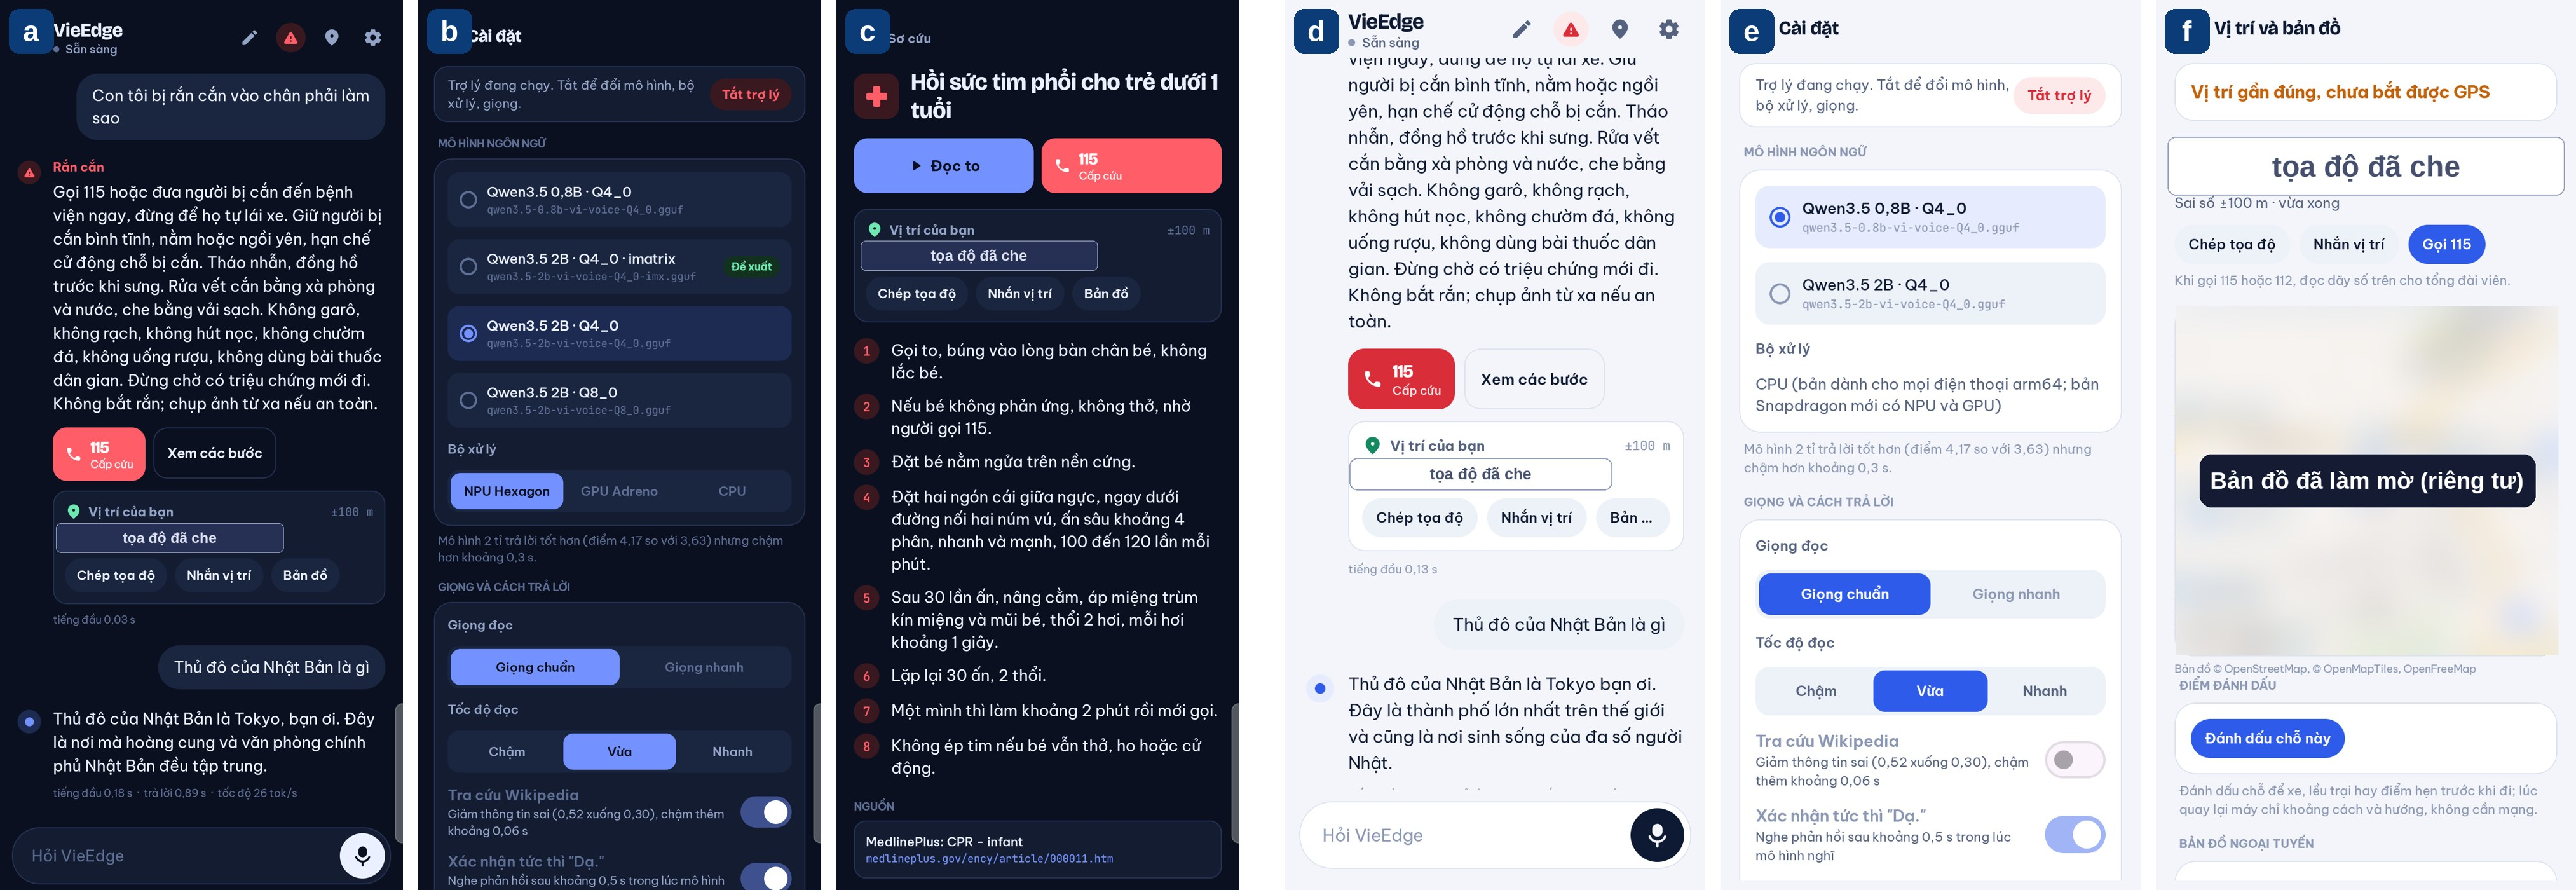
\includegraphics[width=.88\textwidth]{anh_may.jpg}
\caption{Ứng dụng chạy trên thiết bị thực, ảnh chụp màn hình trực tiếp từ thiết bị. Galaxy Z Fold7: (a) câu hỏi khẩn cấp được trả lời bằng thẻ có nút gọi 115 và vị trí, rồi câu hỏi tự do qua LLM; (b) cài đặt, mô hình 2 tỉ trên NPU Hexagon; (c) thẻ hồi sức tim phổi cho trẻ dưới 1 tuổi kèm nguồn. TCL T506T: (d) cùng hai câu hỏi; (e) bản dựng chỉ dùng CPU, mô hình 0,8 tỉ; (f) vị trí và bản đồ ngoại tuyến. Tọa độ được che và bản đồ được làm mờ để bảo vệ thông tin vị trí.}\label{fig:app}
\end{figure*}

\subsection{Những gì đã thử mà không hiệu quả}\label{sec:negative}
Bộ mã hoá (encoder) PhoWhisper-tiny biên dịch được cho Hailo-8L (HEF 19 đến 20\,MB) nhưng độ tương đồng cosine với ONNX chỉ đạt 0,842 khi lượng tử hoá sau huấn luyện và 0,655 sau 6 epoch tinh chỉnh có lượng tử hoá, dưới ngưỡng 0,9 đã đặt ra, nên không được đưa vào đường ống và chưa có WER trên phần cứng Hailo. Giải mã suy đoán~\cite{speculative} không cải thiện tốc độ (13,9 so với 14,3 token/s). Cửa sổ STT thích ứng làm WER tăng gấp đôi (từ 0,158 lên 0,354). Lời nhắc hệ thống yêu cầu trả lời trực tiếp, tự nhiên làm số câu mở đầu bằng ``Mình không chắc'' giảm từ 252 xuống 21 trên 345 câu nói, nhưng tỉ lệ ảo giác tăng từ 0,21 lên 0,48, nên lời nhắc ưu tiên tính trung thực được giữ lại. Gemma-4-E2B có tỉ lệ ảo giác thấp hơn (0,05 với câu văn bản) nhưng trên Fold7 chỉ sinh 8 đến 12 token/s, nội dung trả lời có sau 6 đến 7,5\,s, nên không được sử dụng.

\subsection{Hạn chế}
Toàn bộ độ trễ được đo bằng giọng đọc tổng hợp, chưa có người nói thực; WER của Zipformer trên giọng này là 19\% so với 4\% trên VIVOS, nên chất lượng với người dùng thực có thể khác. Mỗi cấu hình chỉ có 12 đến 16 lượt, đủ phát hiện chênh lệch lớn nhưng chưa đủ cho chênh lệch dưới khoảng 10\%. Việc chấm điểm do một mô hình ngôn ngữ lớn thực hiện, chưa có đánh giá của con người. Các thẻ an toàn chưa được chuyên gia y tế thẩm định và câu thử do nhóm tự soạn; cả hai việc này cần được thực hiện trước khi triển khai thực tế. Thiết bị phổ thông mới được thử trên một mẫu. Hướng tiếp theo quan trọng nhất là thu thập dữ liệu giọng nói thực qua micro điện thoại.

\section{Kết luận}
VieEdge-Voice cho thấy hỏi đáp bằng giọng nói tiếng Việt có thể chạy ngoại tuyến đầu cuối trên thiết bị biên. Trên Pi 5, câu có sẵn được trả lời sau 0,52\,s và câu qua LLM sau khoảng 2 đến 2,4\,s; trên Fold7, mô hình 2 tỉ tham số kèm tra cứu trả lời sau 1,53\,s. Hệ điều hành thời gian thực có giá trị khi cần cô lập lõi xử lý âm thanh, không phải để tăng tốc suy luận. Với câu hỏi khẩn cấp, thẻ có trích dẫn nguồn đáng tin cậy hơn nội dung do mô hình nhỏ sinh ra, và bộ so khớp đơn giản được đánh giá trên tập độc lập cho kết quả tốt hơn nhiều so với để LLM tự chọn thẻ. Ứng dụng cũng chạy được trên điện thoại phổ thông 4\,GB RAM với cùng độ chính xác: phản hồi cho câu khẩn cấp có sau \tclSafeMed\,s, trong khi hỏi đáp tự do chậm hơn đáng kể (\hmAnsT\,s). Hướng phát triển tiếp theo là đánh giá với giọng nói thực và xác định điểm kết thúc phát ngôn dựa trên ngữ nghĩa để giảm thời gian chờ.

\balance
\section{Tài liệu tham khảo}
\vspace{-20pt}
{\footnotesize\setlength{\parskip}{0pt}\raggedright
\begin{thebibliography}{99}\setlength{\itemsep}{1pt}
\bibitem{stivers} T. Stivers et al., Universals and cultural variation in turn-taking in conversation, Proceedings of the National Academy of Sciences, 106(26), pp. 10587-10592, 2009.
\bibitem{whisper} A. Radford, J. W. Kim, T. Xu, G. Brockman, C. McLeavey, I. Sutskever, Robust speech recognition via large-scale weak supervision, Proceedings of ICML, PMLR 202, pp. 28492-28518, 2023.
\bibitem{phowhisper} T.-T. Le, L. T. Nguyen, D. Q. Nguyen, PhoWhisper: automatic speech recognition for Vietnamese, ICLR Tiny Papers, 2024.
\bibitem{chipchat} T. Likhomanenko et al., ChipChat: low-latency cascaded conversational agent in MLX, arXiv:2509.00078, 2025.
\bibitem{melt} S. Laskaridis, K. Katevas, L. Minto, H. Haddadi, MELTing point: mobile evaluation of language transformers, Proceedings of ACM MobiCom, pp. 890-907, 2024.
\bibitem{silero} Silero Team, Silero VAD, github.com/snakers4/silero-vad.
\bibitem{zipformer} Z. Yao et al., Zipformer: a faster and better encoder for automatic speech recognition, Proceedings of ICLR, 2024.
\bibitem{zipvi} hynt, Zipformer-30M-RNNT-6000h, huggingface.co/hynt/Zipformer-30M-RNNT-6000h.
\bibitem{sherpa} k2-fsa, sherpa-onnx, github.com/k2-fsa/sherpa-onnx.
\bibitem{piper} Rhasspy, Piper text-to-speech, github.com/rhasspy/piper.
\bibitem{vits} J. Kim, J. Kong, J. Son, Conditional variational autoencoder with adversarial learning for end-to-end text-to-speech, Proceedings of ICML, PMLR 139, pp. 5530-5540, 2021.
\bibitem{fts5} SQLite Consortium, FTS5 extension, sqlite.org/fts5.html.
\bibitem{rag} P. Lewis et al., Retrieval-augmented generation for knowledge-intensive NLP tasks, Proceedings of NeurIPS, 2020.
\bibitem{llamacpp} G. Gerganov et al., llama.cpp, github.com/ggml-org/llama.cpp, commit 7fe450e19.
\bibitem{lora} E. J. Hu et al., LoRA: low-rank adaptation of large language models, Proceedings of ICLR, 2022.
\bibitem{qwen} Qwen Team, Qwen3.5 model cards, huggingface.co/Qwen.
\bibitem{preemptrt} F. Reghenzani, G. Massari, W. Fornaciari, The real-time Linux kernel: a survey on PREEMPT\_RT, ACM Computing Surveys, 52(1), article 18, 2019.
\bibitem{yocto} The Yocto Project, Reference manual, docs.yoctoproject.org.
\bibitem{vivos} H.-T. Luong, H.-Q. Vu, A non-expert Kaldi recipe for Vietnamese speech recognition system, Proceedings of the WLSI/OIAF4HLT Workshop at COLING, Osaka, pp. 51-55, 2016.
\bibitem{gmmlu} S. Singh et al., Global MMLU: understanding and addressing cultural and linguistic biases in multilingual evaluation, Proceedings of ACL, 2025.
\bibitem{speculative} Y. Leviathan, M. Kalman, Y. Matias, Fast inference from transformers via speculative decoding, Proceedings of ICML, PMLR 202, pp. 19274-19286, 2023.
\end{thebibliography}}

\vspace{4pt}
\noindent\begin{minipage}{\columnwidth}\setlength{\parskip}{0pt}
\textbf{Tác giả chịu trách nhiệm bài viết:}\\
Họ tên: \svmot\\
Đơn vị: \khoa, \truong\\
Email: \emailmot
\end{minipage}
\end{document}
